\section{Variables aléatoires, variables à densité}
\subsection{Notion de mesure}

Le vocabulaire parfois employé ici est celui de l'intégration de Lebesgue. Sans rentrer dans les détails, on emploiera des résultats que l'on peut démontrer avec cette théorie de l'intégration qui permet d'unifier le cas discret avec le cas continu.

\begin{definition}{}{}
	Soit $(\Omega,\mathcal{E})$ un espace probabilisable. Une \trouer{mesure positive} est une fonction $\mu$ définie sur la tribu $\mathcal{E}$ et à valeurs dans $\overline{\R}^+$ telle que :
	\begin{enumerate}
		\item $\mu(\emptyset)=0$
		\item  pour toute famille dénombrable $(A_i)_{i \in \N}$ d'éléments de $\mathcal{E}$ deux à deux disjoints,
		$$\mu\left(\bigcup_{n \in \N} A_n \right) = \sum_{i \in \N} \mu(A_n) \qquad \text{($\sigma$-additivité)}$$
	\end{enumerate}
	
	On dit alors que $(\Omega,\mathcal{E},\mu)$ est un espace mesuré.
\end{definition}

\begin{definition}{}{}
	Soit $(\Omega,\mathcal{E},\mu)$ est un \trouer{espace mesuré} : si de plus $\mu(\Omega)=1$, alors $\mu$ est une \trouer{mesure de probabilité}. 
	
	On notera plus fréquemment une mesure de probabilité $\prob$. Le triplet $(\Omega,\mathcal{E},\prob)$ est alors un espace probabilisé.
\end{definition}

On rappelle que la fonction indicatrice $\textbf{1}_A$ est définie par 
$$\textbf{1}_A(x)=\begin{cases}
1 & \text{ si } x \in A \\
0 & \text{ sinon }
\end{cases}
$$

\paragraph{Exemples de mesures}



\begin{enumerate}
	\item Mesure de comptage : soit $(\Omega,\mathcal{P}(\Omega))$ un espace dénombrable. On définit la mesure $\nu$ pour tout $A \in \mathcal{E}$ par :
	$$\nu(A)=
	\begin{cases}
	\#A & \text{si $A$ est fini} \\
	+\infty & \text{sinon}
	\end{cases}$$
	\item Mesure de Dirac : soit $(\Omega,\mathcal{E})$ un ensemble muni d'une tribu et $a \in \Omega$. On définit la mesure $\delta_a$ pour tout $A \in \mathcal{E}$ par :
	$$\delta_a(A)=
	\begin{cases}
	1 & \text{si $a \in A$} \\
	0 & \text{si $a \notin A$}
	\end{cases}$$
	\item Mesure de probabilité discrète : soit $(\Omega,\mathcal{E})$ un espace muni d'une tribu, $(\omega_k)$ une suite de points de $\Omega$, $(a_k)$ une suite de réels positifs telle que $\sum_k a_k = 1$. Alors 
	$$\prob = \sum_k a_k \delta_{\omega_k}$$
	est une mesure de probabilité sur $\Omega$ : pour tout événement $A \in \mathcal{E}$, $$\prob(A)= \sum_k a_k \delta_{\omega_k}(A) = \sum_k a_k  \textbf{1}_A(\omega_k).$$
	\item Mesure de Lebesgue : pour tout intervalle $I$ de $\R$, $\lambda(I) = \text{\it longueur}(I) \in \overline{\R}_+$.
	\item Mesure absolument continue : si $f:\R\to \R_+$ est une fonction positive intégrable, et pour tout $I$ intervalle de $\R$,
	$$\mu(I) = \int_I f(x) \, dx,$$
alors $\mu$ définit une mesure sur $(\R,\mathcal{B}(\R))$. Les mesures de ce type sont dites absolument continues. On dit alors que $f$ est la {\it densité} de la mesure $\mu$.
\\[1mm]
On remarque que dans le cas où $\int_\R f(x) \, dx = 1$, on a $\mu(\R)=1$, et $\mu$ définit une mesure de probabilité.

\end{enumerate}

\subsection{Intégration par rapport à une mesure}

La notion d'intégrale au sens de Riemann permet d'intégrer des fonctions définies sur $\R$, voire $\R^n$. Nous allons esquisser la construction d'une notion d'intégrale sur tout ensemble pourvu d'une mesure. Il s'agit de l'intégrale au sens de Lebesgue.

\begin{definition}{}{}
	Soit $(\Omega,\mathcal{E})$ un espace probabilisable et $(\R,\mathcal{B}(\R))$ l'ensemble des réels muni de sa tribu borélienne. 
	Une application $f \colon \Omega \to \R $ est dite mesurable si pour tout borélien $A \in \mathcal{B}(\R)$, $f^{-1}(A) \in \mathcal{E}$.
\end{definition}

\noindent
On remarque qu'il s'agit exactement de la notion de variable aléatoire : dans le contexte de l'intégration de fonction, on a coutume d'appeler mesurabilité cette propriété.

\vspace{3mm}

Nous allons introduire l'intégrale d'une fonction $f:\Omega \to \R$ mesurable en commençant par considérer le cas des fonctions indicatrices $\textbf{1}_A$, où $A\in \mathcal{B}(\R)$. Comme le suggère le dessin ci-dessous, il est naturel de définir l'intégrale de la fonction $\textbf{1}_A$ par rapport à la mesure $\mu$ sur $(\Omega,\mathcal{E})$ par
	$$\int \textbf{1}_A \,d\mu = \int_\Omega \textbf{1}_A \,d\mu = \mu(A).$$
\begin{center}
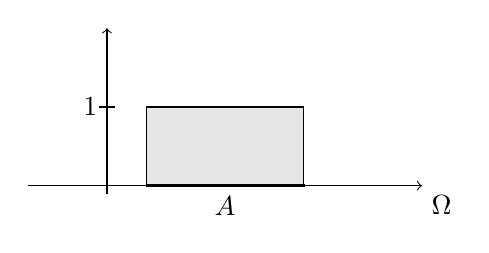
\begin{tikzpicture}
\draw[->] (-1,0) -- (4,0) node[below right] {$\Omega$};
\draw [->] (0,-0.1) -- (0,2);
%\draw [domain=0:3, samples=200] plot(\x,\x>1);
\filldraw [fill=gray!20,draw=black]
(0.5,0) -- (0.5,1) -- (2.5,1) -- (2.5,0) -- cycle;
\draw[very thick] (0.49,0) -- (2.51,0) node[midway,below] {$A$};
\draw (-0.1,1) -- (0.1,1);
\draw (0,1) node[left] {1};
\end{tikzpicture}
\end{center}

Comme nous souhaitons naturellement que l'intégrale par rapport à une mesure ait la propriété de linéarité, cette définition entraîne immédiatement l'expression de l'intégrale de fonctions mesurables du type $\sum_{i=1}^n \alpha_n \textbf{1}_{A_i}$ :
	$$\int \sum_{i=1}^n \alpha_i \textbf{1}_{A_i} d\mu =  \sum_{i=1}^n \alpha_i \mu(A_i).$$
Ces fonctions sont appelées fonctions étagées.




\begin{center}
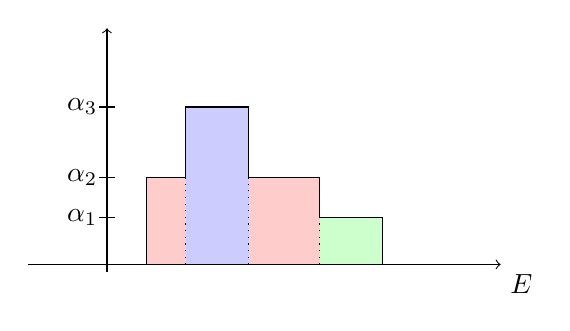
\begin{tikzpicture}
\draw[->] (-1,0) -- (5,0) node[below right] {$E$};
\draw [->] (0,-0.1) -- (0,3);
%\filldraw [fill=gray!20,draw=black]
\fill [fill=red!20] (0.5,0) -- (1,0) -- (1,1.1) -- (0.5,1.1) -- cycle;
\fill [fill=blue!20] (1,0) -- (1,2) -- (1.8,2) -- (1.8,0) -- cycle;
\fill [fill=red!20] (1.8,0) -- (2.7,0) -- (2.7,1.1) -- (1.8,1.1) -- cycle;
\fill [fill=green!20] (2.7,0) -- (3.5,0) -- (3.5,0.6) -- (2.7,0.6) -- cycle;
\draw (0.5,0) -- (0.5,1.1) -- (1,1.1) -- (1,2) -- (1.8,2) -- (1.8,1.1) -- (2.7,1.1) -- (2.7,0.6) -- (3.5,0.6) -- (3.5,0) -- cycle;
\draw[dotted] (1,0) -- (1,1.1);
\draw[dotted] (1.8,0) -- (1.8,1.1);
\draw[dotted] (2.7,0) -- (2.7,0.6);
\draw (-0.1,0.6) -- (0.1,0.6);
\draw (-0.1,1.1) -- (0.1,1.1);
\draw (-0.1,2) -- (0.1,2);
\draw (0,0.6) node[left] {$\alpha_1$};
\draw (0,1.1) node[left] {$\alpha_2$};
\draw (0,2) node[left] {$\alpha_3$};
\end{tikzpicture}
\end{center}


De là, nous pouvons définir l'intégrale de toute fonction mesurable positive $f$ en l'approchant par des fonctions étagées, comme le montre le dessin ci-dessous. On note $\int f d \mu$ cette intégrale, ou encore $\int f(x)\, d\mu(x)$.

Ceci permet finalement de définir l'intégrale de toute fonction intégrable, c'est-à-dire toute fonction $f$ mesurable telle que $\int |f| d\mu<\infty$.


\begin{center}
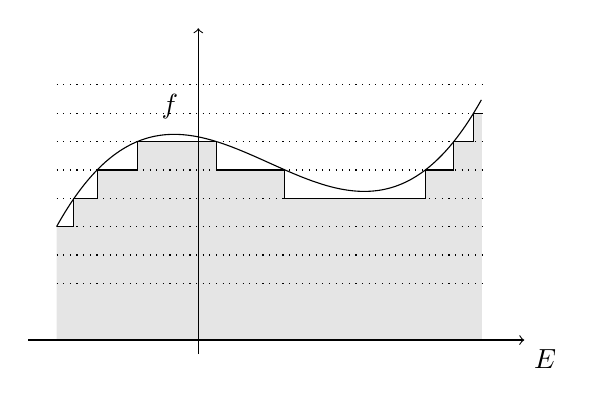
\begin{tikzpicture}[scale=1.8]
\draw [domain=0:3, samples=200] plot(\x,1/3*\x^3-3/2*\x^2+1.8*\x+0.8) ;
\fill [fill=gray!20] 
	(0,0) -- (0,0.8) -- (0.12,0.8) -- (0.12,1) -- (0.29,1) -- (0.29,1.2) -- (0.57,1.2) -- (0.57,1.4) -- (1.13,1.4) -- (1.13,1.2) -- (1.61,1.2) -- (1.61,1)
	-- (2.6,1) -- (2.6,1.2) -- (2.8,1.2) -- (2.8,1.4) -- (2.94,1.4) -- (2.94,1.6) -- (3,1.6) -- (3,0) -- cycle;
\draw (0,0.8) -- (0.12,0.8) -- (0.12,1) -- (0.29,1) -- (0.29,1.2) -- (0.57,1.2) -- (0.57,1.4) -- (1.13,1.4) -- (1.13,1.2) -- (1.61,1.2) -- (1.61,1) -- (2.6,1) -- (2.6,1.2) -- (2.8,1.2) -- (2.8,1.4) -- (2.94,1.4) -- (2.94,1.6) -- (3,1.6);
\foreach \i in {0.4,0.6,0.8,1,1.2,1.4,1.6,1.8}
{\draw[dotted] (0,\i) -- (3,\i);
}
\draw[->] (-0.2,0) -- (3.3,0) node[below right] {$E$};
\draw [->] (1,-0.1) -- (1,2.2);
\draw (0.8,1.65) node {$f$};
\end{tikzpicture}
\end{center}


\begin{definition}{}{}
	Soit $f$ une fonction mesurable définie sur un espace mesuré  $(\Omega,\mathcal{E},\mu)$ et $A \in \mathcal{E}$. Alors $f \times \textbf{1}_A$ est une fonction mesurable et l'intégrale de $f$ sur $A$ par rapport à la mesure $\mu$ est le nombre réel (ou infini) :
	
	$$\int_A f d\mu = \int f \cdot \textbf{1}_A d\mu.$$
\end{definition}


%
%\begin{definition}
%
%	Soit $f=\sum_{i=1}^n \alpha_i \textbf{1}_{A_i}$ une fonction étagée positive définie sur un espace mesuré  $(\Omega,\mathcal{E},\mu)$. Alors l'intégrale de $f$ par rapport à la mesure $\mu$ est le nombre réel (ou infini) :
%	
%	$$\int f d\mu = \int f(x) d\mu(x) = \sum_{i=1}^{n} \alpha_i \mu(A_i) \leq +\infty$$
%\end{definition}
%
%
%
%\begin{definition}
%	Soit $f$ une fonction mesurable positive définie sur un espace mesuré  $(\Omega,\mathcal{E},\mu)$. Alors $f$ est limite simple d'une suite de fonction étagées positives $(f_n)$. L'intégrale de $f$ par rapport à la mesure $\mu$ est le nombre réel (ou infini) :
%	
%	$$\int f d\mu  = \lim\limits_{n \to +\infty} \int f_n d\mu $$
%\end{definition}
%
%Il reste à définir l'intégrale d'une fonction mesurable quelconque. Pour cela, il suffit de définir $f^+=\sup(f,0)$ et $f^-=\sup(-f,0)$ qui sont chacune des fonctions mesurables positives.
%
%\begin{definition}
%	Soit $f$ une fonction mesurable définie sur un espace mesuré  $(\Omega,\mathcal{E},\mu)$. Alors l'intégrale de $f$ par rapport à la mesure $\mu$ est le nombre réel (ou infini) :
%	
%	$$\int f d\mu = \int f^+ d\mu - \int f^- d\mu$$
%\end{definition}


\paragraph{Exemples}

\begin{enumerate}
	\item Mesure de Dirac $\delta_a$, où $a\in \Omega$ : si $f$ est une fonction mesurable, alors
		$$\int f d\delta_a = f(a).$$
	\item Mesure de comptage $\nu$ sur $\N$ : si $f:\N\to \R$, alors
		$$\int f d\nu = \sum_{k=0}^\infty f(k).$$
	\item Mesure de Lebesgue sur $\R$ : on obtient la même notion d'intégrale que celle obtenue avec l'intégrale de Riemann, c'est-à-dire que pour toute fonction Riemann-intégrable,
		$$\int_{[a,b]} f d\lambda = \int_a^b f(x) dx.$$
	\item Mesure absolument continue : si $\mu$ est une mesure absolument continue de densité $g$, alors pour toute fonction $f$ intégrable,
		$$\int f d\mu = \int f(x)g(x) dx.$$
\end{enumerate}

%Si $\mu$ est la mesure de comptage et si $A = \{x_1,...x_n\}$, alors 
%	$$\int \textbf{1}_A d\mu = \mu(A) = n$$
%	
%Si $\mu = \lambda$ est la mesure de Lebesgue et si $A = ]a;b[$, alors 
%$$\int \textbf{1}_A d\lambda = \lambda(A) = b-a = \int_a^b dx$$

%Par passage à la limite sur les fonctions étagées, on définit l'intégrale d'une fonction mesurable positive, puis de signe quelconque, sur une partie mesurable. En particulier, pour la mesure de Lebesgue $\mu =\lambda$, les calculs sont identiques à ceux de l'intégrale de Riemann :
%$$\int_{[a;b]} f(x) \,d\lambda(x) = \int_a^b f(x) \, dx$$
%
%On dit qu'une fonction mesurable $f \colon \Omega \to \R$ est intégrable si 
%$$\int |f| d\mu < +\infty$$

\subsection{Ensembles négligeables et vérités presque sûres}

\begin{definition}{}{}
	Soit $(\Omega,\mathcal{E},\mu)$ un espace mesuré. Un ensemble $A \in \mathcal{E}$ est dit \trouer{négligeable} si $\mu(A)=0$.
\end{definition}

\begin{exemple}{}{}
Si $\mu$ est la mesure de Lebesgue, alors un ensemble $A$ est négligeable si et seulement si $A$ est de longueur nulle.
\end{exemple}

Ainsi, l'ensemble $\{3,5,7\}$ est négligeable pour la mesure de Lebesgue $\lambda$ : en effet, par $\sigma$-additivité, $\lambda(\{3,5,7\}) = \lambda(\{3\})+\lambda(\{5\})+\lambda(\{7\})$. Or $\{3\} = [3;3]$ donc $\lambda(\{3\}) = 3-3 = 0$. De même, $\lambda(\{5\})=\lambda(\{7\})=0$. En revanche, l'ensemble $\{3,5,7\}$ n'est pas négligeable pour la mesure de comptage. 

\begin{definition}{}{}
	Soit $(\Omega,\mathcal{E},\mu)$ un espace mesuré. Une propriété est dite \trouer{vraie presque partout} si elle est vraie sur $\Omega \setminus A$ où $A$ est un ensemble négligeable pour la mesure $\mu$.
\end{definition}

Etant donné $\R$ muni de la mesure de Lebesgue, la fonction $x \mapsto \frac{1}{x}$ est donc continue presque partout sur $\R$ car elle est continue sur $\R \setminus \{0\}$ et $\{0\}$ est négligeable.

\subsection{Lois de probabilité, lois à densité}

On rappelle que si $X$ est une variable aléatoire réelle, sa loi, notée $\prob_X$ est définie par
	$$\prob_X(A)=\prob(X^{-1}(A)) = \prob(X\in A).$$
Comme on l'a vu, $\prob_X$ définit une mesure de probabilité sur $(\R,\mathcal{B}(\R))$.

\begin{exemple}{}{}
Si $X$ est une variable aléatoire discrète, à valeurs dans $\N$, alors pour tout $A\in \mathcal{B}(\R)$,
	$$\prob_X(A)\,=\, \prob(X\in A)\,=\, \sum_{k,~k\in A} \prob(X=k) \,=\, \sum_{k\in \N} \prob(X=k) \,\delta_k(A).$$
Par conséquent, on a en fait $\prob_X = \sum_{k\in \N} \prob(X=k)\,\delta_k$.
\end{exemple}

\begin{definition}{}{}
	Soit $f:\R\to \R^+$ une fonction intégrable. On dit que la variable aléatoire réelle $X$ admet pour densité $f$ si sa loi $\prob_X$ est absolument continue et a $f$ pour densité, c'est-à-dire que pour tout $A\in \mathcal{B}(\R)$, 
	$$\prob_X(A) = \prob(X \in A) = \int_A f d\lambda.$$
	
	On dit alors que $X$ est une variable aléatoire \trouer{absolument continue} ou variable aléatoire \trouer{à densité}. Dans ce cas, on a $$\int_{-\infty}^{+\infty} f(x) dx = 1.$$
\end{definition}

\paragraph{Caractérisation d'une densité de probabilité : } Une fonction $f:\R\to \R$ est une densité de probabilité si $f$ est une fonction positive presque partout sur $\R$ et 
$\int_{-\infty}^{+\infty} f(x) dx = 1$.

\begin{exemple}{}{}
Si $X$ est une variable aléatoire qui désigne le résultat de l'expérience aléatoire qui consiste à choisir au hasard un réel dans l'intervalle $[0;1]$, alors $X$ est une variable à densité, dont la densité est donnée par la fonction $f = \textbf{1}_{[0;1]}$. Si $0\leq a \leq b \leq 1$, on a alors
	$$\prob(a\leq X \leq b) = \prob_X([a;b]) = \int_a^b 1 \, dx = b-a.$$
\end{exemple}

\vspace{3mm}
On remarque que si $X$ est une variable aléatoire à densité, alors pour tout $a\in \R$
	$$\prob(X=a) = \int_a^a f(x) dx = 0.$$
Par conséquent, si $a, b\in \R$ avec $a\leq b$, alors on a  
$$\prob(a\leq X \leq b) = \prob(a<X\leq b) = \prob(a\leq X < b)  = \int_a^b f(x)dx.$$

\begin{exemple}{Variable aléatoire absolument continue}{exvac}
    Soit $f \colon \mathbb{R} \to \mathbb{R}$ définie par : \[
        f(x) = \begin{cases}
            \frac{1}{2} & \text{si } x \in [-1, 1] \\
            0 & \text{sinon}
        \end{cases}
    \]
    
    Voici une représentation graphique :

    \begin{center}
        \begin{tikzpicture}[scale=2]
            % Axes
            \draw[->] (-2.1,0) -- (2.1,0) node[right] {$x$};
            \draw[->] (0,-0.5) -- (0,1.1) node[above] {$f(x)$};
        
            % Function
            \draw[very thick, red] (-1,0.5) -- (1,0.5);
            \draw[very thick, red] (-2,0) -- (-1,0);
            \draw[very thick, red] (1,0) -- (2,0);

            % Dashed lines
            \draw[dashed, red] (-1,0) -- (-1,0.5);
            \draw[dashed, red] (1,0) -- (1,0.5);
        
            % Ticks
            \foreach \x in {-1,1}
            \draw[shift={(\x,0)}] (0pt,2pt) -- (0pt,-2pt) node[below] {$\x$};
        
            \foreach \y in {0.5}
            \draw[shift={(0,\y)}] (2pt,0pt) -- (-2pt,0pt) node[left,yshift=10pt] {$\y$};
        \end{tikzpicture}
    \end{center}

    Alors $f$ est une densité de probabilité. En effet, on a :
    \begin{enumerate}
        \item $f$ est positive ;
        \item $f$ est intégrable et $\int_{-\infty}^{+\infty} f(x) \mathrm{d}x = \int_{-1}^1 \frac{1}{2} \mathrm{d}x = 1$
    \end{enumerate}

    On peut donc définir une variable aléatoire $X$ de densité $f$. On a alors par exemple : \[
        \prob\left(X \in \left[-\frac{3}{4}, -\frac{1}{4}\right]\right) = \int_{-\frac{3}{4}}^{-\frac{1}{4}} f(x) \mathrm{d}x = \int_{-\frac{3}{4}}^{-\frac{1}{4}} \frac{1}{2} \mathrm{d}x = \frac{1}{4}
    \]

    %représentation graphique : (rectangle hachuré entre -3/4 et -1/4)
    \begin{center}
        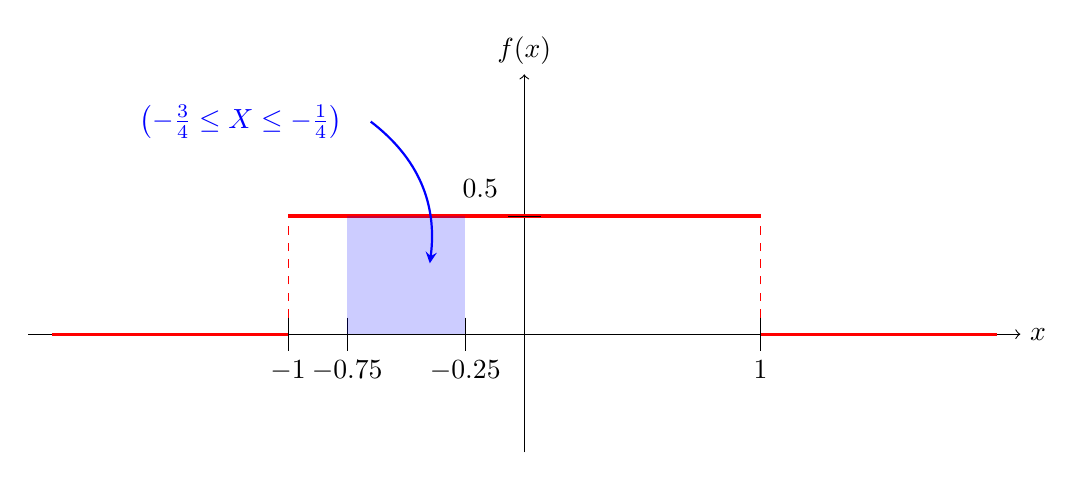
\begin{tikzpicture}[scale=3]
            % Axes
            \draw[->] (-2.1,0) -- (2.1,0) node[right] {$x$};
            \draw[->] (0,-0.5) -- (0,1.1) node[above] {$f(x)$};
        
            % Function
            \draw[very thick, red] (-1,0.5) -- (1,0.5);
            \draw[very thick, red] (-2,0) -- (-1,0);
            \draw[very thick, red] (1,0) -- (2,0);

            % Dashed lines
            \draw[dashed, red] (-1,0) -- (-1,0.5);
            \draw[dashed, red] (1,0) -- (1,0.5);

            % Rectangle
                    
            % Ticks
            \foreach \x in {-1,-0.75,-0.25,1}
            \draw[shift={(\x,0)}] (0pt,2pt) -- (0pt,-2pt) node[below] {$\x$};
        
            \foreach \y in {0.5}
            \draw[shift={(0,\y)}] (2pt,0pt) -- (-2pt,0pt) node[left,yshift=10pt] {$\y$};

            %area 
            \fill[blue, opacity=0.2] (-0.75,0) rectangle (-0.25,0.5);

            %arrow
            \draw[->, >=stealth, line width=0.8pt, bend left, blue] (-0.65,0.90) to (-0.4,0.3);

            %text
            \node[blue] at (-1.2,0.9) {$\prob\left(-\frac{3}{4} \leq X \leq -\frac{1}{4}\right)$};
        \end{tikzpicture}
    \end{center}

\end{exemple}


\subsection{Fonction de répartition}

La définition dans le cas général est donnée au paragraphe \ref{section_fonctionrepartition} du chapitre précédent. 

Si $X$ est une variable aléatoire réelle absolument continue de densité $f$, alors la fonction de répartition $F_X$ est définie pour tout $t \in \R $ par 
$$F_X(t) = \prob(X \leq t) = \int_{-\infty}^{t} f(x)dx$$

\begin{proposition}{}{}
	Soit $X$ une variable aléatoire réelle absolument continue de densité $f$. Alors $F_X$ est continue sur $\R$ et de classe $\mathcal{C}^1$ sur $\R \setminus \{x_1,...,x_p\}$ où $x_1,...,x_p$ sont les points où $f$ n'est pas continue. 

De plus, pour tout $t \in \R \setminus \{x_1,...,x_p\}$, on a
$$F_X'(t) = f(t).$$
\end{proposition}

Cette propriété permet de retrouver la densité d'une variable aléatoire à partir de sa fonction de répartition. Si la fonction de répartition présente des points de non dérivabilité, on en déduit une densité modulo un nombre fini de points. Cela suffit pour caractériser la loi d'une variable aléatoire absolument continue. 

\begin{exemple}{De la fonction de répartition à la densité}{exfoncrepdensite}
	Soit $X$ une variable aléatoire dont la fonction de répartition $F_X$ est définie par : \[
	F_X(t) = \begin{cases}
	0 & \text{si } t < 0 \\
	t^2 & \text{si } t \in [0, 1] \\
	1 & \text{si } t > 1
	\end{cases}
	\]
	
	La fonction $F_X$ est de classe $\mathcal{C}^1$ en tout point sauf en $0$ et $1$. 
	Voici une représentation graphique :
	
	\begin{center}
		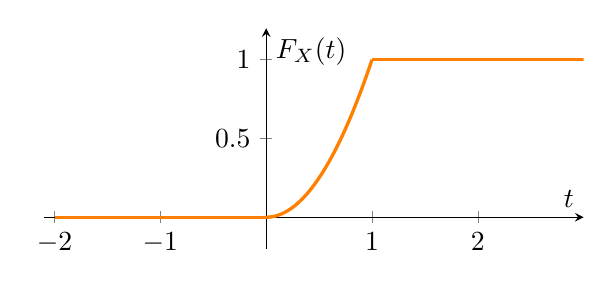
\begin{tikzpicture}
		\begin{axis}[
		axis lines = middle,
		xlabel = $t$,
		ylabel = {$F_X(t)$},
		ymin=-0.2,
		ymax=1.2,
		xmin=-2.1,
		xmax=3,
		xtick={-2,-1,0,1,2},
		ytick={0,0.5,1},
		yticklabels={0, 0.5, 1},
		no marks,
		y=2cm,
		]
		\addplot [
		domain=-2:0, 
		samples=100, 
		color=orange,
		very thick,
		]
		{0};
		\addplot [
		domain=0:1, 
		samples=100, 
		color=orange,
		very thick,
		]
		{x^2};
		\addplot [
		domain=1:3, 
		samples=100, 
		color=orange,
		very thick,
		]
		{1};
		\end{axis}
		\end{tikzpicture}
	\end{center}
	
	On a $\forall t \in \mathbb{R}\setminus \{0,1\}$ : \[
	f(t) = F_X'(t) = \begin{cases}
	0 & \text{si } t < 0 \\
	2t & \text{si } t \in ]0, 1[ \\
	0 & \text{si } t > 1
	\end{cases}
	\]
	
	Une fonction densité est définie modulo un nombre fini de points. On peut donc définir une fonction densité $f$ de $X$ par : $\forall x \in \mathbb{R}$ : \[
	f(x) = \begin{cases}
	0 & \text{si } x < 0 \\
	2x & \text{si } x \in [0, 1] \\
	0 & \text{si } x > 1
	\end{cases}
	\]
	
	Voici une représentation graphique : 
	
	\begin{center}
		\begin{tikzpicture}[scale=2]
		% Axes
		\draw[->] (-2.1,0) -- (2.1,0) node[right] {$x$};
		\draw[->] (0,-0.5) -- (0,2.1) node[above] {$f(x)$};
		
		% Function
		\draw[very thick, red] (-2,0) -- (0,0);
		\draw[very thick, red] (0,0) -- (1,2);
		\draw[very thick, red] (1,0) -- (2,0);
		% Dashed lines
		\draw[dashed, red] (1,2) -- (1,0);
		% Ticks
		\foreach \x in {-1,1}
		\draw[shift={(\x,0)}] (0pt,2pt) -- (0pt,-2pt) node[below] {$\x$};
		
		\foreach \y in {0.5,1,1.5,2}
		\draw[shift={(0,\y)}] (2pt,0pt) -- (-2pt,0pt) node[left] {$\y$};
		\end{tikzpicture}
	\end{center}
	
	Pour calculer la probabilité de l'événement $\{0{,}5 < X \leq 1{,}5\}$, on a deux méthodes possibles : 
	\begin{enumerate}
		\item Avec la fonction de répartition : \[
		\prob(0{,}5 < X \leq 1{,}5) = F_X(1{,}5) - F_X(0{,}5) = 1 - 0{,}5^2 = 0{,}75 
		\]
		\item Avec la densité : \[
		\prob(0{,}5 < X \leq 1{,}5) = \int_{0{,}5}^{1{,}5} f(x) \mathrm{d}x = \int_{0{,}5}^{1} 2x \mathrm{d}x = \left[ x^2 \right]_{0{,}5}^1 = 0{,}75
		\]
	\end{enumerate}
\end{exemple}

 Réciproquement :

\begin{proposition}{}{}
	Soit $F$ est une fonction réelle :
	\begin{enumerate}
		\item continue sur $\R$ ;
		\item croissante sur $\R$ ;
		\item $\lim\limits_{-\infty} F = 0$ et $\lim\limits_{+\infty} F = 1$ ;
		\item de classe $\mathcal{C}^1$ sur $\R \setminus \{x_1,...,x_p\}$.
	\end{enumerate}
	alors il existe une variable aléatoire $X$ absolument continue dont $F$ est la fonction de répartition.
\end{proposition}

\begin{figure}[h!]
	\centering
	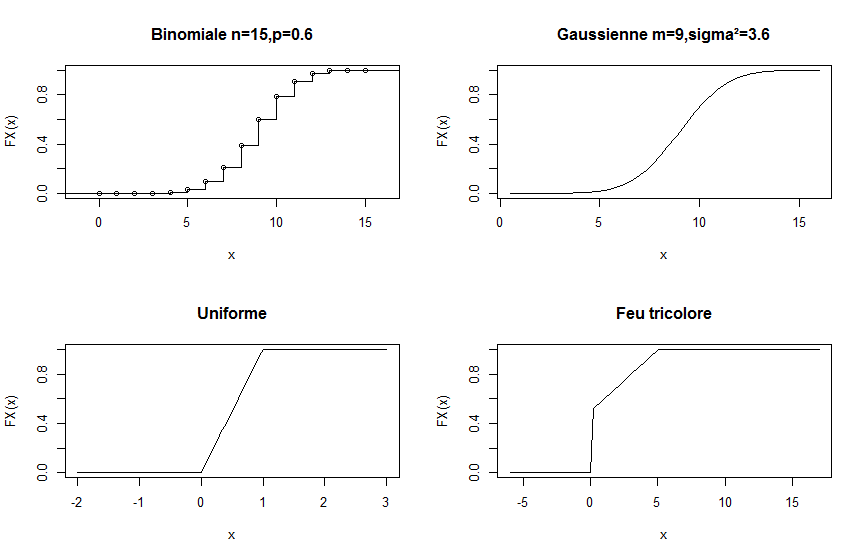
\includegraphics[width=0.9\linewidth]{FonctionRepartition}
	\caption{Exemples de fonctions de répartition de variables aléatoires discrètes, absolument continues et mixtes.}
	\label{fig:fonctionrepartition}
\end{figure}

Dans l'exemple suivant, on représente une fonction de répartition d'une variable aléatoire qui n'est ni discrète, ni absolument continue. 

\begin{center}
	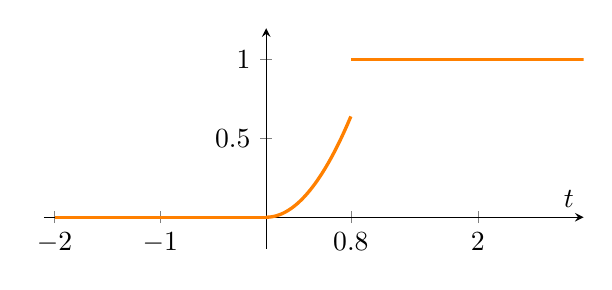
\begin{tikzpicture}
	\begin{axis}[
	axis lines = middle,
	xlabel = $t$,
	%ylabel = {$F_X(t)$},
	ymin=-0.2,
	ymax=1.2,
	xmin=-2.1,
	xmax=3,
	xtick={-2,-1,0,0.8,2},
	ytick={0,0.5,1},
	yticklabels={0, 0.5, 1},
	no marks,
	y=2cm,
	]
	\addplot [
	domain=-2:0, 
	samples=100, 
	color=orange,
	very thick,
	]
	{0};
	\addplot [
	domain=0:0.8, 
	samples=100, 
	color=orange,
	very thick,
	]
	{x^2};
	%ajouter un petit rond au point de coordonnées (0.75,0.75^2)
	\addplot [
	domain=0.8:3, 
	samples=100, 
	color=orange,
	very thick,
	]
	{1};
	\end{axis}
	\end{tikzpicture}
\end{center}

Cette fonction est discontinue en $x=0.8$ donc la variable aléatoire associée n'est pas absolument continue. De plus, elle n'est pas associée à une variable aléatoire discrète car elle n'est pas en escalier. On peut lire $\prob(X=0.8)$ sur la fonction de répartition, c'est le saut de discontinuité en $x=0.8$, c'est-à-dire $\prob(X=0.8)= F(0.8) - F(0.8^-)$. 

\subsection{Espérance}

Nous donnons ici une définition de l'espérance plus générale que la définition de la partie précédente, qui repose sur la notion d'intégrale par rapport à une mesure de probabilité.

\begin{definition}{}{}
	Soient $(\Omega,\mathcal{E},\prob)$ est un espace probabilisé, $X \colon \Omega \to \R $ une variable aléatoire. On définit l'espérance de $X$ par 
	$$\EX = \int_\Omega X \,d\prob$$	
lorsque cette intégrale est bien définie.
\end{definition}

Pour calculer l'espérance d'une variable aléatoire, on a le plus souvent recours au théorème de transfert ci-dessous, qui permet d'écrire $\EX$ comme une intégrale sur $\R$ au lieu de $\Omega$.

\begin{theoreme}{de transfert}{}
Soient $X$ un variable aléatoire réelle et $\phi:\R\to \R^+$ une fonction mesurable. Alors 	
	$$\mathbb{E}(\phi(X)) = \int_\R \phi(x) \, dP_X(x).$$
En particulier, $\displaystyle \mathbb{E}(X) = \int_\R x \, dP_X(x)$
\end{theoreme}

\paragraph{Exemples importants}
\begin{enumerate}
\item Cas d'une variable aléatoire $X$ discrète à valeurs dans $\N$ : $\prob_X = \sum_{k\in \N} \prob(X=k)\delta_k$. On retrouve donc la définition de la partie précédente :
	$$\EX = \int x \, dP_X (x) = \sum_{k\in \N} \prob(X=k) \int x\, d\delta_k(x) = \sum_{k\in \N} k \,\prob(X=k).$$
Plus généralement, si $X(\Omega) = \{x_i\}_i$, alors $\displaystyle \EX = \sum_i x_i \, \prob(X=x_i)$.
\item Cas d'une variable aléatoire $X$ absolument continue : si on note $f$ la densité de $X$, alors l'intégration par rapport à une mesure à densité donne
	$$\EX = \int x \, dP_X(x) = \int_{-\infty}^{+\infty} x f(x)\, dx.$$
Plus généralement, pour toute fonction positive $\phi$,
	$$\mathbb{E}(\phi(X)) = \int_{-\infty}^{+\infty} \phi(x) f(x)dx.$$
\end{enumerate}

\begin{definition}{}{}
	Si $\EX = 0$, la variable $X$ est dite \trouer{centrée}. 
\end{definition}

Par linéarité, on remarque que pour toute variable aléatoire $X$, la variable $Y=X - \EX$ est centrée.

\begin{definition}{Moment}{}
	Soit $(\Omega,\mathcal{E},\prob)$ est un espace probabilisé, $X \colon \Omega \to \R $ une variable aléatoire. Alors $\mathbb{E}(X^n)$ est le \trouer{moment} d'ordre $n$ de $X$.
\end{definition}

\begin{proposition}{}{}
	D'après le théorème de transfert, $X$ admet un moment d'ordre $n$ si et seulement si la fonction $x \mapsto x^n$ est intégrable pour la mesure $d\prob_X$ et on a 
	$$\mathbb{E}(X^n) = \int_\Omega X^n \, d\prob = \int_{\R}^{} x^n \, d\prob_X(x)$$
\end{proposition}


\subsection{Variance}

\begin{definition}{Variance et écart-type}{}
	Soit $X \colon (\Omega,\mathcal{E}) \to (E,\mathcal{F})$ une variable aléatoire admettant un moment d'ordre 2. Alors la \trouer{variance} de $X$ est le réel
	$$\var(X)=\mathbb{E}\left((X-\EX)^2\right)$$
	
	L'\trouer{écart-type} de $X$ est 
	$$\sigma(X)=\sqrt{\var(X)}$$
\end{definition}

\begin{definition}{}{}
	Une variable $X$ telle que $\sigma(X)=1$ est une variable \trouer{réduite}. 
\end{definition}

\begin{proposition}{}{}
	Soit $X$ une variable aléatoire d'espérance $\mu$ et d'écart-type $\sigma$. Alors la variable $Z=\frac{X-\mu}{\sigma}$ est une variable centrée réduite.
\end{proposition}

\begin{proposition}{Formule de König-Huygens}
	Soit $X$ une variable aléatoire admettant un moment d'ordre 2. Alors 
	$$\var(X)=\mathbb{E}(X^2)-\left(\EX\right)^2$$
\end{proposition}

Cette propriété permet de calculer plus facilement une variance en utilisant le théorème de transfert.

\begin{proposition}{}{}
	Soit $X$ une variable aléatoire. Alors
	\begin{enumerate}
		\item pour tout $\lambda \in \R $ :  $\var(\lambda X)= \lambda^2 \var(X)$ et $\var(X+\lambda)=\var(X)$.
		\item Si $\var(X)=0$ alors $X$ est une variable constante presque sûrement, i.e. elle est constante avec probabilité 1.
	\end{enumerate}
\end{proposition}



\subsection{Changement de variable aléatoire}

Soit $X$ une variable aléatoire absolument continue dont on connaît la loi (donc la densité que l'on notera $f$) et $Y=\phi(X)$ une variable aléatoire ($\phi$ est mesurable). On cherche à identifier la loi de $Y$. 

\paragraph{Méthode 1 :} on exprime sa fonction de répartition $F_Y$.

\begin{enumerate}
	%	\item La fonction de répartition de $X$ est $F_X$ définie par $F_X(t)=\int_{-\infty}^{t}f(x)dx$.
	\item Par définition, $F_Y(t)= \prob(Y \leq t) = \prob(\phi(X) \leq t)$
	\item Or l'événement $\{\phi(X) \leq t\}$ se réécrit aussi $\{\phi(X) \in ]-\infty;t]\} =  \{X \in \phi^{-1}(]-\infty;t])\}$
	\item Par définition, $f$ est la densité de $X$ donc $\prob(X \in A) = \int_A f(x)dx$ pour tout événement $A$. En posant $A = \phi^{-1}(]-\infty;t])$, on obtient donc une expression de $F_Y(t) = \int_{\phi^{-1}(]-\infty;t])} f(x)dx$
	\item On écrit sous la forme $F_Y(t)= \int_{-\infty}^{t}g(x)dx$ et on en déduit que $Y$ est une variable aléatoire absolument continue de densité $g$.
\end{enumerate}

	
\paragraph{Méthode 2 :} on utilise le théorème d'identification :
	
\begin{theoreme}{Identification}{}
		Soit $X$ une variable aléatoire réelle à densité telle que pour toute fonction continue bornée $h$, , 
		$$\mathbb{E}(h(X))=\int_{\R}^{}h(x)f(x)dx$$
		
		Alors $f$ est la densité de la variable aléatoire $X$.
\end{theoreme}

Ce théorème s'utilise de la manière suivante : étant donné un changement de variable $\phi(X)$, on exprime $\mathbb{E}(h(\phi(X)))$ pour une fonction bornée $h$ quelconque à l'aide du théorème de transfert,  puis on effectue le changement de variables $u=\phi(x)$ dans l'intégrale pour mettre le résultat sous la forme $\mathbb{E}(h(\phi(X))) = \int_{\R}^{}h(u)g(u)du$, de sorte que l'expression $g(u)$ obtenue donne la densité de la variable $\phi(X)$ par application du théorème d'identification.
	
	\begin{exemple}{}{}
Soit $X$ une variable aléatoire absolument continue dont la densité est donnée par $$f(x)=\frac{1}{2}\textbf{1}_{[-1;1]}(x)$$
	Pour déterminer la loi de $Y=X^2$ à l'aide du théorème d'identification, on exprime pour toute fonction continue bornée $h$ (dite fonction <<muette>>) la quantité $\mathbb{E}(h(Y))$ en utilisant le théorème de transfert appliqué à $\phi(X) = h(X^2)$ :
	
\begin{align*}
\mathbb{E}(h(X^2)) &= \int_{\R} h(x^2) f(x) dx \\
&= \int_{\R} h(x^2) \frac{1}{2}\textbf{1}_{[-1;1]}(x) dx \\
&= \int_{-1}^1 h(x^2) \frac{1}{2} dx \\
&= 2\int_0^1 h(x^2) \frac{1}{2} dx \text{ par parité } \\
&= \int_0^1 h(x^2) dx
\end{align*} 
En effectuant le changement de variables $u=x^2$ de $[0;1]$ dans $[0;1]$, on a $dx = \frac{1}{2\sqrt{u}}du$ d'où 
\begin{align*}
\mathbb{E}(h(X^2)) &= \int_0^1 h(u) \frac{1}{2\sqrt{u}}du \\
&= \int_{\mathbb{R}}^{} h(u) \frac{1}{2\sqrt{u}} \textbf{1}_{[0;1]}(u) du
\end{align*}

Ceci étant vrai pour toute fonction bornée $h$, on déduit du théorème d'identification que la variable $X^2$ admet pour densité la fonction $g(x) = \frac{1}{2\sqrt{x}} \textbf{1}_{[0;1]}(x)$. 
	\end{exemple}
	
	\section{Lois usuelles}
	On décrit ci-dessous plusieurs lois usuelles pour des variables aléatoires réelles $X$ absolument continues, donc admettant une densité notée $f$.
	
	\subsection{Loi uniforme}
	La loi uniforme sur un intervalle $[a;b]$ est définie par :
	
	\paragraph{Densité :} 
	$$f(x)=\frac{1}{b-a} \textbf{1}_{[a;b]}(x)$$

\begin{center}
	\begin{tikzpicture}[scale=2]
	% Define the variables
	\def\a{-0.7}
	\def\b{0.5}
	\pgfmathsetmacro{\h}{1/(\b-\a)} % Density height
	
	% Axes
	\draw[->] (-2.1,0) -- (2.1,0) node[right] {$x$};
	\draw[->] (0,-0.5) -- (0,1.5) node[above] {$f(x)$};
	
	% Function
	\draw[ultra thick, red] (\a,\h) -- (\b,\h);
	\draw[ultra thick, red] (-2,0) -- (\a,0);
	\draw[ultra thick, red] (\b,0) -- (2,0);
	
	% Dashed lines
	\draw[dashed, red] (\a,0) -- (\a,\h);
	\draw[dashed, red] (\b,0) -- (\b,\h);
	
	% Ticks
	\foreach \x in {\a}
	\draw[shift={(\x,0)}] (0pt,2pt) -- (0pt,-2pt) node[below] {$a$};
	
	\foreach \x in {\b}
	\draw[shift={(\x,0)}] (0pt,2pt) -- (0pt,-2pt) node[below] {$b$};
	
	\foreach \y in {\h}
	\draw[shift={(0,\y)}] (2pt,0pt) -- (-2pt,0pt) node[left,yshift=10pt] {$\frac{1}{b-a}$};
	\end{tikzpicture}
	
\end{center}
	
	\paragraph{Fonction de répartition :}
	
$$ F(t)= \begin{cases} 0 & \text{ si } t<a, \\ 
\frac{t-a}{b-a} & \text{ si } t\in]a;b[, \\
1 & \text{ si } t\geq b
\end{cases} $$

    \begin{center}
	\begin{tikzpicture}[scale=2]
	% Define the variables
	\def\a{-0.7}
	\def\b{0.5}
	
	% Axes
	\draw[->] (-2.1,0) -- (2.1,0) node[right] {$t$};
	\draw[->] (0,-0.5) -- (0,1.5) node[above] {$F_X(t)$};
	
	% Function
	\draw[ultra thick, orange] (-2,0) -- (\a,0);
	\draw[ultra thick, orange] (\a,0) -- (\b,1);
	\draw[ultra thick, orange] (\b,1) -- (2,1);
	
	% Ticks
	\foreach \x in {\a}
	\draw[shift={(\x,0)}] (0pt,2pt) -- (0pt,-2pt) node[below] {$a$};
	
	\foreach \x in {\b}
	\draw[shift={(\x,0)}] (0pt,2pt) -- (0pt,-2pt) node[below] {$b$};
	
	\foreach \y in {1}
	\draw[shift={(0,\y)}] (2pt,0pt) -- (-2pt,0pt) node[left] {$\y$};
	\end{tikzpicture}
\end{center}
	\paragraph{Paramètres :}
	
	$$\EX = \frac{a+b}{2} \qquad V(X)=\frac{(b-a)^2}{12}$$
	
	\subsection{Loi exponentielle}
	La loi exponentielle de paramètre $\lambda >0$ est définie par :
	
	\paragraph{Densité :} 
	$$f(x)=\lambda e^{-\lambda x} \textbf{1}_{[0;+\infty[}(x)$$
	\begin{center}
		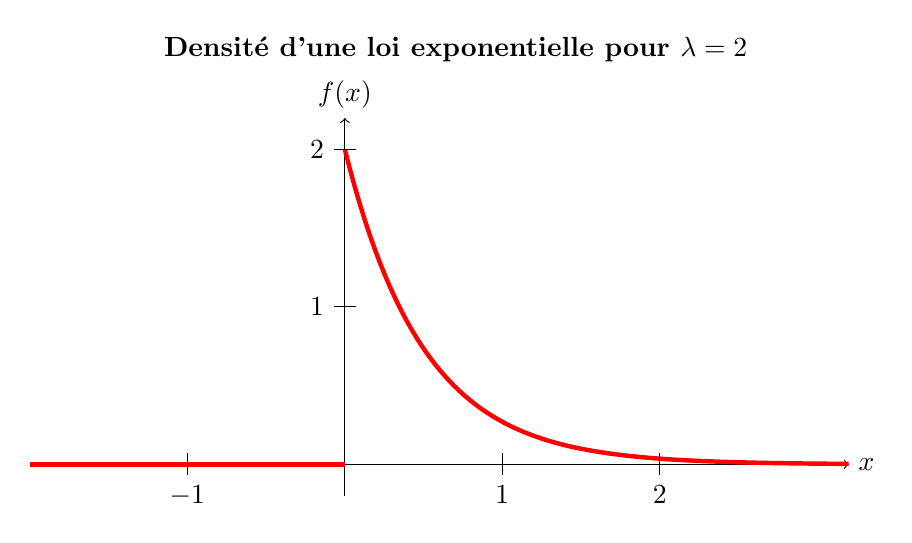
\begin{tikzpicture}[scale=2, domain=0:3.2, samples=100]
		% Define the variables
		\def\l{2} % lambda
		
		% Axes
		\draw[->] (-0.2,0) -- (3.2,0) node[right] {$x$};
		\draw[->] (0,-0.2) -- (0,2.2) node[above] {$f(x)$};
		
		% Function
		\draw[ultra thick, red, smooth] plot (\x, {\l*exp(-\l*\x)});
		\draw[ultra thick, red] (-2,0) -- (0,0);
		
		% Ticks
		\foreach \x in {-1,1,2}
		\draw[shift={(\x,0)}] (0pt,2pt) -- (0pt,-2pt) node[below] {$\x$};
		
		\foreach \y in {1,2}
		\draw[shift={(0,\y)}] (2pt,0pt) -- (-2pt,0pt) node[left] {$\y$};
		
		% Title
		\node[above, font=\bfseries] at (current bounding box.north) {Densité d'une loi exponentielle pour $\lambda=2$};
		\end{tikzpicture}
	\end{center}
	
	\paragraph{Fonction de répartition :}
	
$$ F(t)= \begin{cases} 0 & \text{ si } t<0, \\ 
1-e^{-\lambda t} & \text{ si } t \geq 0
\end{cases} $$
	\begin{center}
		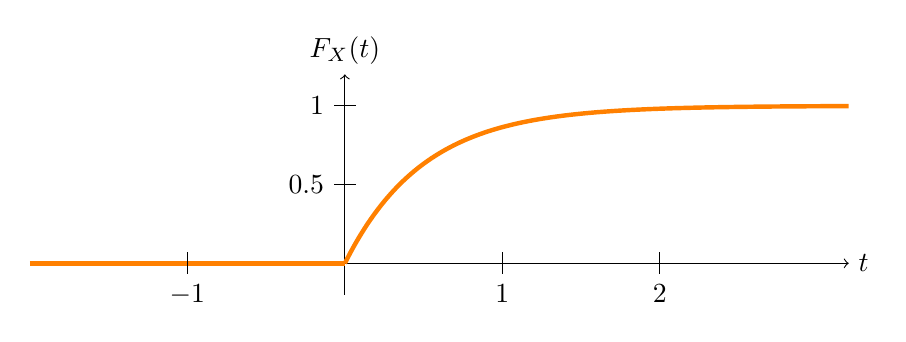
\begin{tikzpicture}[scale=2, domain=0:3.2, samples=100]
		% Define the variables
		\def\l{2} % lambda
		
		% Axes
		\draw[->] (-0.2,0) -- (3.2,0) node[right] {$t$};
		\draw[->] (0,-0.2) -- (0,1.2) node[above] {$F_X(t)$};
		
		% Function
		\draw[ultra thick, orange, smooth] plot (\x, {1-exp(-\l*\x)});
		\draw[ultra thick, orange] (-2,0) -- (0,0);
		
		% Ticks
		\foreach \x in {-1,1,2}
		\draw[shift={(\x,0)}] (0pt,2pt) -- (0pt,-2pt) node[below] {$\x$};
		
		\foreach \y in {0.5,1}
		\draw[shift={(0,\y)}] (2pt,0pt) -- (-2pt,0pt) node[left] {$\y$};
		\end{tikzpicture}
	\end{center}
	\paragraph{Paramètres :}
	
	$$\EX = \frac{1}{\lambda} \qquad V(X)=\frac{1}{\lambda^2}$$
	
	\begin{theoreme}{}{}
		La loi exponentielle est une loi sans mémoire : pour tout $(n,m) \in \N^2$, 
		$$\prob_{X>m}(X > m+n)=\prob(X>n)$$
	\end{theoreme}

La loi exponentielle permet en particulier de modéliser des temps d'attente. 
%	\begin{center}
%		\begin{figure}[h!]
%			\psset{xunit=4cm,yunit=2cm,plotpoints=200,algebraic=true}
%			\begin{pspicture*}(-0.75,-0.05)(3,3)
%			\multido{\n=2+1,\iblue=20+5}{5}{%
%				\psplot[linecolor=blue!\iblue,linewidth=2pt]{0}{5}{\n*EXP(-\n*x)}    }
%			\psaxes[Dy=1,ticksize=0 3pt]{->}(0,0)(3,3)
%			\end{pspicture*}
%			\caption{Courbes de densité d'une loi exponentielle $\mathcal{E}(\lambda)$ pour $\lambda \in \{2,...,7\}$}
%		\end{figure}
%	\end{center}
	
	\subsection{Loi normale centrée réduite :}
	
	La densité suivante définit la loi normale centrée réduite :
	
	$$f(x)=\frac{1}{\sqrt{2\pi}}\;\; \mathrm{e}^{-\frac{x^2}{2}}$$
		
\begin{center}
	
	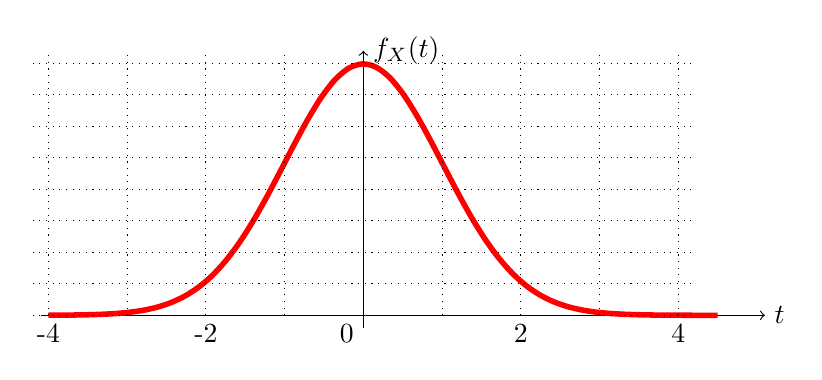
\begin{tikzpicture}[domain=-4:4.5,yscale=8]
		\draw[->] (-4.1,0) -- (5.1,0) node[right] {$t$};
		\draw[->] (0,-0.02) -- (0,0.42) node[right] {$f_X(t)$};
		%	\filldraw[draw=blue,fill=blue!20] 	(0.5,0) node[below]{$a$} -- plot[domain=0.5:2,smooth] (\x,{0.399*exp(-((\x)^2)/2)}) --	(2,0) node[below]{$b$} -- cycle;
		%	\draw (1.2,0.12)--(3,0.2)node[above right]{$P(a \leq X \leq b)$};    
		\draw[color=red,smooth,line width=2pt,samples=50] plot (\x,{0.399*exp(-((\x)^2)/2)});
		\draw [ystep=0.05,dotted](-4.2,0) grid (4.2,0.42);
		\path (0,0) node [below left]{0};
		\path (4,0) node [below]{4};
		\path (2,0) node [below]{2};
		\path (-4,0) node [below]{-4};
		\path (-2,0) node [below]{-2};
		%	\path (0,0.1) node [left]{0,1};
	\end{tikzpicture}
	
\end{center}

\begin{proposition}{Propriétés de la loi normale centrée réduite}{proploinormale}
	Soit $Z$ une variable aléatoire suivant la loi normale centrée réduite $\mathcal{N}(0,1)$. Alors :
	\begin{enumerate}
		\item $\E(Z) = 0$ ;
		\item $\var(Z) = 1$.
	\end{enumerate}
	De plus, on a que 
	$$\prob(Z \geq 0) = \prob(Z \leq 0) = \frac{1}{2}$$
\end{proposition}

\begin{proof}
	On a : \[
	\E(Z) = \int_{-\infty}^{+\infty} x f(x) \mathrm{d}x = \int_{-\infty}^{+\infty} x \frac{1}{\sqrt{2\pi}} e^{-\frac{x^2}{2}} \mathrm{d}x = 0 \text{ car la fonction intégrée est impaire}
	\]
	De plus, on a : 
	\begin{align*}
	\E(Z^2) & = \int_{-\infty}^{+\infty} x^2 f(x) \mathrm{d}x \\
	& = \int_{-\infty}^{+\infty} x^2 \frac{1}{\sqrt{2\pi}} e^{-\frac{x^2}{2}} \mathrm{d}x \\
	& = 0 - \int_{-\infty}^{+\infty} -\frac{1}{\sqrt{2\pi}} e^{-\frac{x^2}{2}} \mathrm{d}x \text{ par intégration par parties} \\
	& = 1
	\end{align*}
	
	D'après la formule de Huygens, on a : \[
	\var(Z) = \E(Z^2) - \E(Z)^2 = 1 - 0 = 1
	\]
	Enfin, on a : \[
	\prob(Z \geq 0) = \int_0^{+\infty} \frac{1}{\sqrt{2\pi}} e^{-\frac{x^2}{2}} \mathrm{d}x = \frac{1}{2}  = 	\int_{-\infty}^0 \frac{1}{\sqrt{2\pi}} e^{-\frac{x^2}{2}} \mathrm{d}x = \prob(Z \leq 0)
	\]
\end{proof}

\importantbox{ La fonction $x \mapsto \frac{1}{\sqrt{2\pi}} e^{-\frac{x^2}{2}}$ n'a pas de primitive que l'on peut écrire avec des fonctions usuelles. 

Les calculs de probabilité se font donc, sauf cas particuliers, à l'aide de tables de valeurs ou de logiciels de calcul contenant ces tables.}

Plus précisément, ce sont les valeurs de la fonction de répartition d'une variable $Z \sim \mathcal{N}(0, 1)$ qui sont tabulées. On note $\Phi$ la fonction de répartition d'une variable $Z \sim \mathcal{N}(0, 1)$. On a donc : $$
\Phi(t) = \prob(Z \leq t)
$$

Voici une représentation graphique : 

\begin{center}
	\begin{tikzpicture}[yscale = 2]
	% Axes
	\draw[->] (-3.1,0) -- (3.1,0) node[right] {$t$};
	\draw[->] (0,-0.2) -- (0,1.2) node[above] {$\Phi(t)$};
	% Ticks
	\foreach \x in {-2,-1,0,1,2}
	\draw[shift={(\x,0)}] (0pt,1pt) -- (0pt,-1pt) node[below] {$\x$};
	\foreach \y in {0.5}
	\draw[shift={(0,\y)}] (2pt,0pt) -- (-2pt,0pt) node[left] {$\frac{1}{2}$};
	\foreach \y in {1}
	\draw[shift={(0,\y)}] (2pt,0pt) -- (-2pt,0pt) node[left] {$\y$};
	\draw[orange,ultra thick] plot[domain=-3:3,samples=100] (\x,{0.5*(1+erf(\x/sqrt(2)))});
	\end{tikzpicture}
\end{center}


Le principe général pour calculer une probabilité avec une loi normale centrée réduite est le suivant : 
\begin{enumerate}
	\item On ramène l'événement à un événement de la forme $\{Z \leq t\}$ où $Z \sim \mathcal{N}(0, 1)$ et $t>0$ ; pour cela, on peut utiliser : 
	\begin{enumerate}
		\item la symétrie de la loi normale : $\prob(Z \geq t) = \prob(Z \leq -t)$ ;
		\item le complémentaire : $\prob(Z \geq t) = 1 - \prob(Z \leq t)$ ;
	\end{enumerate}
	\item On utilise les tables de la fonction de répartition de $Z$ pour calculer la probabilité $\prob(Z \leq t)$.
\end{enumerate}



	\subsection{Loi normale}
	La loi normale (ou loi gaussienne) $\mathcal{N}(\mu,\sigma)$ de paramètres $\mu \in \R$ et $\sigma >0$ est définie par :
	
	\paragraph{Densité :} 
	$$f(x)=\frac{1}{\sigma \sqrt{2\pi}} e^{-\frac{(x-\mu)^2}{2\sigma^2}}$$
	
	
	
	\begin{proposition}{}{}
	Si $X$ suit une loi normale  $\mathcal{N}(\mu,\sigma)$, alors :
	$$\EX = \mu \qquad \var(X)=\sigma^2$$
\end{proposition}
	

	
	\begin{proposition}{}{}
		Si $X$ suit une loi normale  $\mathcal{N}(\mu,\sigma)$, alors :
		$$Z = \frac{X-\mu}{\sigma}$$
		suit une loi normale  $\mathcal{N}(0,1)$.
	\end{proposition}

	\begin{exemple}{Calculs de probabilité pour une loi $\mathcal{N}(\mu,\sigma)$}{excalculprobaNmusigma}
		Soit $X$ une variable aléatoire suivant la loi normale $\mathcal{N}(2, 3)$. On veut réaliser le calcul de probabilité suivant :
		\begin{align*}
			\prob(-4 \leq X \leq 8) &= \prob\left(\frac{-4 - 2}{3} \leq \frac{X - 2}{3} \leq \frac{8 - 2}{3}\right) \\
			&= \prob\left(-2 \leq \frac{X - 2}{3} \leq 2\right) \\
			&= \prob\left(\frac{X - 2}{3} \leq 2\right) - \prob\left(\frac{X - 2}{3} \leq -2\right) \\
			&= \prob\left(Z \leq 2\right) - \prob\left(Z \leq -2\right) \text{ avec $Z \sim \mathcal{N}(0, 1)$} \\
			&= \Phi(2) - \Phi(-2) \\
			&= \Phi(2) - (1 - \Phi(2)) \\
			&= 2\Phi(2) - 1 \\
			&\approx 0{,}9545
		\end{align*}
		\begin{center}
			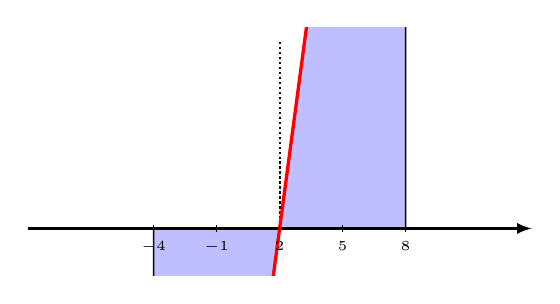
\begin{tikzpicture}[xscale=0.8,yscale=6]
				\def\mu{2}
				\def\sigma{3}
				\def\bornegauche{\fpeval{(-4-\mu)/\sigma}}
				\def\bornedroite{\fpeval{(8-\mu)/\sigma}}
				\clip (-4,-0.1) rectangle (4,0.425);
			 %   \draw (0, 0) node[below] {$2$};
			 %   \draw (1, 0) node[below] {$\fpeval{2+3*1}$};
			 
				\draw[black, semithick, fill = blue!25] (\bornegauche,0) -- plot [domain=\bornegauche:\bornedroite,samples=100] (\x,{\densnorm{\x}}) -- (\bornedroite,0) -- cycle;
				\draw[thick,->,>=latex] (-4,0) -- (4,0) ;
				\draw[thick,densely dotted] (0,0) -- (0,0.398942280401433);
				\draw[very thick,domain=-4:4,samples=100,smooth,red] plot (\x,{\densnorm{\x}});
			%thicks
				\foreach \x in {-2,-1,0,1,2}
				\draw[shift={(\x,0)}] (0pt,0.2pt) -- (0pt,-0.2pt) node[font=\tiny,below] {$\fpeval{2+3*\x}$};
			\end{tikzpicture}
			\end{center}
	\end{exemple}
	
	\subsection{Loi de Cauchy}
	La loi de Cauchy de paramètres $x_0 \in \R $ et $\lambda >0$ est définie par :
	
	\paragraph{Densité :} 
	$$f(x) = \frac{\lambda}{\pi((x-x_0)^2+\lambda^2)}$$
	
	Elle apparaît par exemple en spectroscopie pour modéliser des raies d'émission. C
	
	\paragraph{Fonction de répartition :}
	
	$$F_X(t)=\frac{1}{\pi} \arctan{\left(\frac{x-x_0}{\lambda}\right)} + \frac12$$
	
	Cette loi a la particularité de ne pas admettre d'espérance finie, ni d'écart type. La loi des grands nombres ne s'applique pas à cette loi.
	
	\paragraph{Paramètres :}
	
	$$\EX = \text{non défini} \qquad \var(X)= \text{non défini}$$
	

	
\section{Couples de variables aléatoires}
	
	\subsection{Quelques prérequis techniques}
	
	\begin{theoreme}{Fubini}{}
		Soit $f$ une fonction mesurable positive sur $\mathbb{R}^2$. Alors les fonctions $x \mapsto \int_{\mathbb{R}} f(x,y)\mathrm{d}y$ et $y \mapsto \int_{\mathbb{R}} f(x,y)dx$ sont mesurables et 
		$$\int_{\mathbb{R}} \left( \int_{\mathbb{R}}  f(x,y) \mathrm{d}x  \right) \mathrm{d}y = \int_{\mathbb{R}} \left( \int_{\mathbb{R}}  f(x,y) \mathrm{d}y  \right) \mathrm{d}x$$
		Le résultat est alors noté 
		$$ \iint_{\mathbb{R}^2} f(x,y)\, \mathrm{d}x\mathrm{d}y$$ 
	\end{theoreme}
	
	\begin{exemple}{}{}
		On souhaite calculer l'intégrale 
		$$I=\iint_D f(x,y)\,\mathrm{d}x\mathrm{d}y$$
		où $f(x,y)=x+y$ et $D = \{ (x,y) \mid x\ge0,x^2\le y\le1\}$.
		Le théorème de Fubini permet donc d'écrire 
		
		$$I = \iint_{\mathbb{R}^2} 1_{[0;1]}(x)  1_{[x^2;1]}(y) (x+y) \mathrm{d}x\,\mathrm{d}y = \int_0^1\left(\int_{x^2}^1(x+y)\,\mathrm{d}y\right)\,\mathrm{d}x $$
				
		Pour $x \in [0;1]$ fixé, on calcule la première intégrale par rapport à $y$ :
		$$\int_{x^2}^1(x+y)\,\mathrm{d}y=\left[xy + \frac{y^2}2\right]^{1}_{x^2}=x + \frac12- x^3 - \frac{x^4}2$$
		Il reste à calculer la seconde intégrale par rapport à $x$ :
		$$I=\int_0^1 \left(x + \frac12- x^3 - \frac{x^4}2\right) \; \mathrm{d}x =  \frac{13}{20}$$
		
		De manière équivalente, on peut exprimer le domaine d'intégration de la manière suivante :
		$$D= \{ (x,y) \mid y \in [0;1] \, , \, x \in [0~;~\sqrt{y}]\} $$
		ce qui invite à utiliser le théorème de Fubini pour écrire l'intégrale :
		$$I = \int_0^1\left(\int_0^{\sqrt{y}} (x+y){d}x\right)\,{d}y$$
		On intègre donc d'abord par rapport $x$, puis par rapport à $y$, puis on obtient le même résultat.
	\end{exemple}
	
	\begin{theoreme}{Changement de variables}{}
		Soit $f$ une fonction d'un ouvert $O \subset \mathbb{R}^d$ dans $\mathbb{R}^k$, mesurable, intégrable. Soit $\varphi$ un $\mathcal{C}^1$-difféomorphisme de $O$ dans un ouvert $O' \subset \mathbb{R}^d $. Alors 
		$$\int_{O} f(x)dx = \int_{O'} f\left(\varphi^{-1}(u)\right)|\det Jac_{\varphi^{-1}}(u)|\mathrm{d}u$$
		
		où $Jac_{\varphi^{-1}}=
		\begin{pmatrix} 
		\dfrac{\partial {\varphi^{-1}}_1}{\partial u_1} & \cdots & \dfrac{\partial {\varphi^{-1}}_1}{\partial u_d} \\
		\vdots & \ddots & \vdots \\
		\dfrac{\partial {\varphi^{-1}}_d}{\partial u_1} & \cdots & \dfrac{\partial {\varphi^{-1}}_d}{\partial u_d}
		\end{pmatrix}.$
	\end{theoreme}
	
	\begin{exemple}{changement de variables en coordonnées polaires}{}
		Ce changement de variables s'écrit pour tout $(x,y) \in \R^2 \backslash \{(0;0)\}$ et $(r,\theta) \in \R_+^* \times ]0;2\pi[$.
		$$(x,y)=\Phi(r,\theta)=(r\cos\theta,r\sin\theta)$$
		
		La matrice jacobienne de $\Phi$ au point $(r,\theta)$ s'écrit :
		$$Jac_{\Phi}(r,\theta) =
		\begin{pmatrix}
		\cos\theta & -r\sin\theta \\
		\sin\theta &  r\cos\theta \\
		\end{pmatrix}.$$
		La valeur absolue du déterminant de la matrice jacobienne est $r >0$. Cela donne :
		
		$$\int_{O} f(x,y)dxdy = \int_{O'} f\left(r\cos\theta,r\sin\theta\right)r\mathrm{d}r\mathrm{d}\theta$$
	\end{exemple}
	
	\subsection{Densité d'un couple de variables aléatoires}
	\begin{definition}{}{}
		Soit $(X,Y)$ un couple de variables aléatoires $(\Omega,\prob) \to \R^2$. Le couple de variables $(X,Y)$ admet une \trouer{densité} s'il existe une fonction $f \colon \R^2 \to \R^+$ telle que pour tout événement $A$, 
		$$\prob((X,Y) \in A) = \int_A f(x,y)\,\mathrm{d}\lambda(x,y)$$
		où $\mathrm{d}\lambda$ est la mesure de Lebesgue sur $\R^2$. 
	\end{definition}
	

	
	\begin{proposition}{}{}
   Si $(X,Y)$ est un couple de variables aléatoires admettant une densité $f \colon \R^2 \to \R^+$ alors $X$ et $Y$ admettent également une densité et les lois marginales de $(X,Y)$ sont déterminées par :
	\begin{itemize}
		\item densité de $X$ : $f_X \colon x \mapsto \int_{\R}^{} f(x,y)dy$
		\item densité de $Y$ : $f_Y \colon y \mapsto\int_{\R}^{} f(x,y)dx$
	\end{itemize}
	\end{proposition}	
		
Réciproquement, si $X$ et $Y$ admettent chacune une densité, cela n'implique pas forcément que $(X,Y)$ admette une densité. Par exemple, si $X$ admet une densité, il en est de même pour $-X$, alors que le couple $(X,-X)$ prend ses valeurs dans la droite $D=\{(x,y) \in \R^2, y=-x\}$ qui est de mesure nulle dans $\R^2$. On aurait donc $\prob((X,-X) \in D) = 1$ d'une part et si $(X,-X)$ admettait une densité $f$, alors $\prob((X,-X) \in D) = \int_D f(x,y)dxdy = 0$ car $\lambda(D)=0$.
		

		
		\subsection{Fonction de répartition}
		
		On étend la définition d'une fonction de répartition à un couple de variables aléatoires $(X,Y)$ : c'est la fonction définie sur $\R^2$ par 
		$$F_{(X,Y)} \colon (t_1,t_2) \mapsto \prob(X \leq t_1, Y \leq t_2)$$
		
		Si de plus le couple $(X,Y)$ admet une densité $f$, alors 
		$$F_{(X,Y)}(t_1,t_2) = \int_{-\infty}^{t_1} \left( \int_{-\infty}^{t_2} f(u,v)dv \right) du =  \int_{-\infty}^{t_2} \left( \int_{-\infty}^{t_1} f(u,v)du \right) dv$$
		
		\subsection{Espérance}
		
		\begin{definition}{}{}
			Soit $(X,Y)$ un couple de variables aléatoires admettant une densité $f$. On définit l'espérance $\mathbb{E}(X,Y)=(\EX, \mathbb{E}(Y))$.
			
			Pour toute fonction $h \colon \R^2 \to \R $ mesurable, $h(X,Y)$ est une variable aléatoire et
			$$\mathbb{E}(h(X,Y)) =   \int_{\R^2} h(x,y) f(x,y)dxdy$$
			
			En particulier, 
			
			$$\EX = \int_{\R^2} x f(x,y)dxdy$$
			$$\mathbb{E}(Y) = \int_{\R^2} y f(x,y)dxdy$$
			
			
		\end{definition}
		
		\begin{exemple}{}{}
			Avec $h(x,y)=xy$, on obtient ce calcul :
			$$\mathbb{E}(XY) = \int_{\R^2} xy f(x,y)dxdy$$
			utile pour calculer une covariance.
		\end{exemple}
		
		\subsection{Changement de variables}
		\begin{theoreme}{Identification}{}
			Soit $(X,Y)$ un couple de variables aléatoires réelles tel que pour toute fonction continue bornée $h$,  
			$$\mathbb{E}(h(X,Y))=\int_{\R^2}^{}h(x,y)f(x,y)dxdy$$
			
			Alors $f$ est la densité du couple $(X,Y)$.
		\end{theoreme}
		

		\subsection{Covariance}
		
		\begin{definition}{Covariance}
			Soit un couple de variable aléatoires $(X,Y)$ : la \trouer{covariance} de $X$ et $Y$ est le réel 
			$$\cov(X,Y) = \mathbb{E} \left[ (X-\EX)(Y-\mathbb{E}(Y)) \right] = \mathbb{E}(XY)-\mathbb{E}(X)\mathbb{E}(Y)$$
		\end{definition}
		
		
%		\begin{definition}
%			Si  $cov(X,Y)=0$, alors on dit que $X$ et $Y$ sont \trouer{non linéairement corrélées}.
%		\end{definition}
%		
		
		\begin{proposition}{}{}
			Soit un couple de variable aléatoires $(X,Y)$ et $a,b$ deux réels :
			$$\var(aX+bY)=a^2\var(X)+b^2\var(Y)+2ab \times \cov(X,Y)$$
		\end{proposition}
		
		
		
		\begin{proposition}{}{}
			Soit un couple de variable aléatoires $(X,Y)$ admettant chacune un moment d'ordre 2. Alors 
			$$\cov(X,Y)^2 \leq \var(X)\var(Y)$$	
			
		\end{proposition}
		
		\begin{definition}{Coefficient de corrélation linéaire}{}
			Soit un couple de variable aléatoires $(X,Y)$ admettant chacune un moment d'ordre 2 et des variances non nulles. Alors le coefficient de corrélation linéaire est 
			
			$$\rho(X,Y)=\frac{\cov(X,Y)}{\sqrt{\var(X)\var(Y)}}$$
		\end{definition}
		
		Le coefficient $\rho(X,Y)$ mesure le degré de dépendance linéaire des variables $X$ et $Y$. Il est compris entre $-1$ et $1$. Plus précisément :
		
		\begin{proposition}{}{}
			Soit un couple de variable aléatoires $(X,Y)$ admettant chacune un moment d'ordre 2 et des variances non nulles. Alors $|\rho(X,Y)|=1$ si et seulement s'il existe trois réels $(a,b,c) \neq (0,0,0)$ tels que $aX+bY+c = 0$.
		\end{proposition}
		
		\subsection{Indépendance}
		\begin{definition}{}{}
			Soit $(X,Y)$ un couple de variables aléatoires définies sur un espace $\Omega$. Alors $X$ et $Y$ sont \trouer{indépendantes} si pour tout événement $A$, $B$ alors
			$$\prob(X \in A, Y \in B)=\prob(X \in A) \times \prob(Y \in B)$$
			
			On note aussi $\prob(X \in A, Y \in B) = \prob(\{X \in A\} \cap \{Y \in B\})$
		\end{definition}
		
		\begin{proposition}{}{}
			Soit $(X,Y)$ un couple de variables aléatoires indépendantes, $F_X$ la fonction de répartition de $X$, $F_Y$ la fonction de répartition de $Y$.
			
			Alors la fonction de répartition $F_{(X,Y)}$ du couple $(X,Y)$ est définie pour tout $(t_1,t_2) \in \R^2$ par 
			$$F_{(X,Y)}(t_1,t_2) = F_X(t_1) \times F_Y(t_2)$$
		\end{proposition}
		
		\begin{proposition}{}{}
			Soit $(X,Y)$ un couple de variables aléatoires absolument continues admettant respectivement pour densité $f$ et $g$. Alors $X$ et $Y$ sont indépendantes si et seulement si $(X,Y)$ admet une densité $h$ et pour tout $(x,y) \in \R^2$, 
			$$f(x)g(y)=h(x,y)$$
		\end{proposition}
		
		\begin{proposition}{}{}
			Soit $(X,Y)$ un couple de variables aléatoires admettant chacune une espérance. Si $X$ et $Y$ sont indépendantes, alors 
			$$\EX \mathbb{E}(Y) = \mathbb{E}(XY)$$
		\end{proposition}
		
		On en déduit que si $X$ et $Y$ sont indépendantes, alors $\cov(X,Y)=0$. Attention, la réciproque est fausse.
		

\subsection{Somme de variables aléatoires indépendantes}
		
		\begin{proposition}{}{}
			Soit $(X,Y)$ un couple de variables aléatoires absolument continues et indépendantes. Soit $f$ une densité de $X$ et $g$ une densité de $Y$. Alors la variable $S = X+Y$ admet pour densité la fonction $h$ définie par 
			$$h= f \star g$$
			où $\star$ est le produit de convolution. On rappelle que $f \star g \colon s \mapsto \int_{\R} f(s-x)g(x)dx$
		\end{proposition}
		\begin{proof}
		Par indépendance, la densité du couple $(X,Y)$ est la fonction $(x,y) \mapsto f(x)g(y)$. D'après le théorème de transfert, pour toute fonction continue bornée $\phi$,
		$$\mathbb{E}(\phi(X+Y)) = \iint \phi(x+y)\,f(x)\,g(y)dxdy$$
		On effectue le changement de variable $$(u,v)=(x+y,y)$$ (c'est une bijection de classe $\mathcal{C}^1$). La réciproque s'écrit $(x,y)=(u-v,v)$. La matrice jacobienne est $\begin{pmatrix}
		1 & -1 \\
		0 & 1 \\
		\end{pmatrix} $ et la valeur absolue de son déterminant est $1$. On peut donc écrire $dx\,dy=du\,dv$ et on a finalement  :
	\begin{align*}
	\mathbb{E}(\phi(X+Y)) &=  \iint \phi(u)f(u-v)g(v)du\,dv \\
	&= \int \phi(u) \left( \int f(u-v) g(v)dv \right)du \text{ d'après le théorème de Fubini} \\
	&= \int \phi(u) f\star g(u) du
	\end{align*}
On conclut par le théorème d'identification.
		\end{proof}

		
		\begin{proposition}{}{}
			Si $X_1$ et $X_2$ sont deux variables aléatoires indépendantes, $X_1 \hookrightarrow \mathcal{N}(\mu_1,\sigma_1)$, $X_2 \hookrightarrow \mathcal{N}(\mu_2,\sigma_2)$ alors la somme $S=X_1+X_2$ suit une loi normale $\mathcal{N}(\mu_1 + \mu_2,\sqrt{\sigma_1^2 + \sigma_2^2})$.
		\end{proposition}
		
		\subsection{Minimum et maximum}
		
		Soit $(X,Y)$ un couple de variables aléatoires. On pose $U=\min(X,Y)$ et $V=\max(X,Y)$. Pour étudier la loi de $U$ ou $V$, il est classique de calculer leur \trouer{fonction de répartition} et de remarquer les faits suivants :
		
		\begin{itemize}
			\item $\{\min(X,Y) \geq t\} = \{X \geq t\} \cap \{Y \geq t\}$
			\item $\{\min(X,Y) \leq t\} = \{X \leq t,X \leq Y\} \cup \{Y \leq t,X>Y\}$
			\item $\{\max(X,Y) \leq t\} = \{X \leq t\} \cap \{Y \leq t\}$
			\item $\{t_1 \leq \min(X,Y) \} \cap \{\max(X,Y) \leq t_2\} = \{t_1 \leq X \leq t_2\} \cap \{t_1 \leq Y \leq t_2\}$
		\end{itemize}
		

		
		\subsection{Fonction génératrice des moments}
		
		\begin{definition}{}{}
			Soit $X \colon \Omega \to \R $ une variable aléatoire absolument continue à valeurs dans $\R$ .  La \trouer{fonction génératrice des moments} de X est la série entière définie sur $[-1;1]$ par :
			$$M_X(t)=\mathbb{E}[e^{tX}] =\int e^{tx}f(x)dx$$
			
		\end{definition}
		

		
		\begin{proposition}{}{}
			Si $X$ a pour fonction génératrice $M_X$ et possède un moment d'ordre $n$ alors 
			$$\mathbb{E}(X^n) = M_X^{(n)}(0)$$
		\end{proposition}
		
				\begin{proposition}{Fonction génératrice d'une somme}{}
					Soit  $(X,Y)$ un couple de variables aléatoires réelles. Si $X$ et $Y$ sont indépendantes, alors Pour tout $t \in \R $
					
					$$ M_{X+Y}(t)=M_X(t)M_Y(t)$$

					
				\end{proposition}
		\subsection{Fonction caractéristique}
		
		\begin{definition}{}{}
			La \trouer{fonction caractéristique} d'une variable aléatoire réelle $X$ est la fonction à valeurs complexes définie sur $\R$ par
			
			$$\phi_{X}(t) =\mathbb{E}\left[e^{i tX}\right]$$
		\end{definition}
	
			Si $X$ est une variable aléatoire absolument continue admettant une densité $f$, alors 
			
			$$\phi_{X}(t) = \int_{\R}^{} e^{i tx} f(x)dx$$
			
			Si $(X,Y)$ est un couple de variables aléatoires absolument continues admettant une densité $f$, alors 
			$$\phi_{(X,Y)}(t_1,t_2) = \int_{\R}^{} e^{i (t_1x+t_2y)} f(x,y)\,dx\,dy$$

		

		
		\begin{exemple}{}{}
			Soit $X$ une variable aléatoire suivant une :
			\begin{enumerate}
				\item loi uniforme sur $[-a;a]$ : 
				$$\phi_{X}(t) = \frac{\sin(a t)}{a t}$$
				\item loi normale centrée réduite : 
				$$\phi_{X}(t) = e^{-\frac{t^2}{2}}$$
				\item loi exponentielle de paramètre $\lambda$ :
				$$\phi_{X}(t) = \frac{\lambda}{\lambda - i t}$$
				\item loi binomiale $\mathcal{B}(n,p)$ :
				$$\phi_{X}(t) = (1+p(e^{i t}-1))^n$$
			\end{enumerate}
		\end{exemple}
		
		\begin{proposition}{}{}
			Si $X$ admet une espérance alors $$\EX = -i\phi_X'(0)$$
		\end{proposition}
		
		Une fonction caractéristique détermine la loi :
		
		\begin{proposition}{}{}
			Si $X$ et $Y$ sont deux variables aléatoires telles que $\phi_X=\phi_Y$ alors $X$ et $Y$ suivent une même loi de probabilité.
		\end{proposition}
		
		Pour retrouver la densité $f_X$ d'une variable aléatoire $X$ à partir de sa fonction caractéristique, on peut appliquer la formule d'inversion de Fourier (admise) :

		$$ f_{X}(x)  = \displaystyle \frac{1}{2\pi} \int_{\R} \phi_{X}(t) e^{-i xt} dt $$
		
		\begin{proposition}{Fonction caractéristique d'une somme}{}
			Soit  $(X,Y)$ un couple de variables aléatoires réelles. Si $X$ et $Y$ sont indépendantes, alors pour tout $t \in \R $ :
			
			
			$$ \phi_{X+Y}(t)=\phi_X(t)\phi_Y(t)$$
		%	$$ \phi_{(X,Y)}(t_1,t_2)=\phi_X(t_1)\phi_Y(t_2)$$
			
		\end{proposition}
	
	La réciproque est fausse en général.
	
\section{Simulation de lois}
L'objectif principal de ce paragraphe est d'étudier des méthodes permettant de simuler une variable aléatoire par ordinateur, ou en d'autres termes : comment faire en sorte qu'un ordinateur donne des nombres au hasard ?

Ce n'est pas possible, néanmoins, il existe des algorithmes qui permettent de générer des suites de nombres approchant un tirage hasardeux. Il suffit que les nombres obtenus donnent des résultats satisfaisants à divers tests statistiques pour que l'on puisse supposer qu’ils sont aléatoires. On parle dans ce cas de générateurs pseudo-aléatoires, puisque malgré tout, un algorithme, forcément déterministe, est utilisé. 

\textbf{Dans la suite de ce paragraphe, on supposera acquise la simulation d'une loi uniforme sur $[0;1]$.}

%\subsection{Simulation d'une loi uniforme}

\subsection{Méthode d'inversion de la fonction de répartition}
\begin{theoreme}{}{}
	Soit $X$ une variable aléatoire suivant une loi de probabilités de fonction de répartition $F$. On pose, pour tout $u \in]0;1[$,
	
	$$G(u)=\inf \{x\in \R ; F(x)\geq u \}$$
	
	Soit $U$ une variable aléatoire suivant une loi uniforme sur $[0;1]$. Alors la fonction de répartition de la variable $G(U)$ est $F$.
\end{theoreme}
\begin{proof}
	Ce résultat est admis dans le cas général. Voici une démonstration sous l'hypothèse où $F$ est continue et strictement croissante sur $\R$. 
	
	 Soit la variable aléatoire $Y=F(X)$. On cherche à démontrer que $Y$ suit une loi uniforme sur $[0;1]$. 

Pour cela, on cherche la fonction de répartition de la variable aléatoire $Y$. Soit $t\in\mathbb{R}$. Par définition :
\[ F_Y(t)=\mathbb{P}(Y\leq t)
=\mathbb{P}(F(X)\leq t).
\]
Or la fonction de répartition $F$ prend ses valeurs dans $[0;1]$. On en déduit
\begin{align*}
F_Y(t)=\begin{cases}
0 & \text{ si } t< 0 \\
1 & \text{ si } t\geq 1
\end{cases}
\end{align*}
Soit $t\in[0;1[$. Comme la fonction de répartition $F$ est croissante et supposée continue sur $\mathbb{R}$, il existe au moins un réel $t_0$ tel que $F(t_0)=t$. Alors on a
\begin{align*}
F_Y(t)&=\mathbb{P}(F(X)\leq t) \\
&=\mathbb{P}(F(X)\leq F(t_0)) \\
&=\mathbb{P}(X\leq t_0) \quad \text{ car $F$ est croissante sur $\mathbb{R}$} \\
&=F(t_0) \\
&=t.
\end{align*}
On a ainsi obtenu 
\begin{align*}
F_Y(t)=\begin{cases}
0 & \text{ si } t< 0 \\
t & \text{ si } t\in[0;1[ \\
1 & \text{ si } t\geq 1
\end{cases}
\end{align*}
qui correspond à la fonction de répartition de la loi uniforme sur $[0;1]$. Donc $Y\sim \mathcal{U}([0;1])$.
\end{proof}

\begin{exemple}{simulation d'une loi exponentielle}{}
	La fonction de répartition d'une loi exponentielle $\mathcal{E}(\lambda)$ est 
	$$F(x) = \begin{cases}1-e^{-\lambda x} & \text{ si } x \geq 0 \\
	0 & \text{ sinon }
	\end{cases}$$
	Cette fonction est continue et strictement croissante de $]0;+\infty[$ dans $]0;1[$ donc la fonction $G$ est sa réciproque, elle est définie sur $]0;1[$ par $G \colon u \mapsto -\frac{1}{\lambda}\ln(1-u)$. Ainsi, si $U$ suit une loi uniforme sur $[0;1]$, alors $-\frac{1}{\lambda}\ln(1-U)$ suit une loi exponentielle $\mathcal{E}(\lambda)$. 
	
	Sachant que $1-U$ suit également une  loi uniforme sur $[0;1]$, on peut conclure que $-\frac{1}{\lambda}\ln(U)$ suit une loi exponentielle $\mathcal{E}(\lambda)$. 
\end{exemple}

\begin{exemple}{simulation d'une loi de Bernoulli}{}
	La fonction de répartition d'une loi de Bernoulli $\mathcal{B}(p)$ est 
	$$F(t) = \begin{cases}
	0  & \text{ si } t<0  \\
	1-p & \text{ si } 0 \leq t < 1 \\
	1 & \text{ si } t>1
	\end{cases}$$
	
	Dans ce cas, $\inf\{t\in \R ;  F(t)\geq u \} = \lfloor u+p \rfloor$
	
	Donc si $U$ suit une loi uniforme sur $[0;1]$, alors $\lfloor U+p \rfloor$ suit une loi de Bernoulli  $\mathcal{B}(p)$. 
\end{exemple}

\subsection{Méthode de Box-Müller}
Pour simuler une loi normale, on peut utiliser le théorème central limite  qui permet d'affirmer qu'en additionnant un grand nombre de tirages indépendants, on obtient des résultats distribués approximativement selon une loi normale. 

Il existe des méthodes plus performantes, dont la méthode de Box-Muller qui permet de simuler un couple de variables normales indépendantes. 

\begin{proposition}{}{}
	Soit \((U_1 , U_2)\) un couple de variables aléatoires indépendantes
	identiquement distribuées suivant toutes deux la loi uniforme standard
	\(\mathcal U ([0;1])\)
	
	Alors les variables aléatoires
	\(X = \sqrt{-2 \ln (U_1)} \cos (2 \pi U_2)\) et
	\(Y = \sqrt{-2 \ln (U_1)} \sin (2 \pi U_2)\) sont indépendantes
	identiquement distribuées suivant toutes deux la loi normale centrée
	réduite \(\mathcal N (0;1)\)
\end{proposition}
\begin{proof}
	Une preuve possible est le changement de variables en coordonnées polaires et est laissée en exercice.
\end{proof}




